\documentclass [11pt,twoside]{article}
\usepackage[utf8]{inputenc}
\usepackage[T1]{fontenc}
\usepackage{import}
\documentclass [11pt,twoside]{article}
\usepackage[utf8]{inputenc}
\usepackage[T1]{fontenc}

%Page margins, header and footer positions
\usepackage{geometry}
 \geometry{
 a4paper,
 % total={210mm,297mm},
 left=25mm,
 right=25mm,
 top=30mm,
 bottom=25mm,
 headsep=7mm}

\interfootnotelinepenalty=10000

%To display filling dots in the TOC for all entries
\usepackage[titles]{tocloft}
\renewcommand{\cftsecleader}{\cftdotfill{\cftdotsep}}

%Define new header and footer style
\usepackage{fancyhdr}

\pagestyle{fancy}
\fancyhf{}
\lhead{\color{Gray}{\small{Travlendar+ project by YOUR NAMES}}}
\lfoot{\textcolor{Gray}{\small{Copyright © 2017, YOUR NAMES – All rights reserved}}}
\rfoot{\textcolor{Gray}{\thepage}}
\renewcommand{\headrulewidth}{0pt}

%PACKAGES
\usepackage{wasysym}
\usepackage{pifont}

\newcommand{\supported}{\ding{52}\xspace}
\newcommand{\unsupported}{\ding{55}\xspace}
\newcommand{\partsupported}{\textcolor{black!40}{\ding{52}}\xspace}
\newcommand{\lowsupported}{\textcolor{black!20}{\ding{52}}\xspace}
\newcommand{\unknowsupported}{\textbf{?}\xspace}

%Font: Times
\usepackage{times}
%Change monospaced font
\renewcommand{\ttdefault}{lmtt}

%tables
%\usepackage{tabu}
\usepackage{tabularx}
\usepackage{ltablex}
\usepackage{longtable}
\usepackage{float} % To allow the use of H modifier in long tables

%landscape mode
\usepackage{pdflscape}
\usepackage{rotating}
\usepackage{caption}

%make landscape mode be sensitive to even and odd pages
%start
\def\myrotate{\ifodd\c@page\else-\fi 90}
\makeatletter
\global\let\orig@begin@landscape=\landscape%
\global\let\orig@end@landscape=\endlandscape%
\gdef\@true{1}
\gdef\@false{0}
\gdef\landscape{%
    \global\let\within@landscape=\@true%
    \orig@begin@landscape%
}%
\gdef\endlandscape{%
    \orig@end@landscape%
    \global\let\within@landscape=\@false%
}%
\@ifpackageloaded{pdflscape}{%
    \gdef\pdf@landscape@rotate{\PLS@Rotate}%
}{
    \gdef\pdf@landscape@rotate#1{}%
}
\let\latex@outputpage\@outputpage
\def\@outputpage{
    \ifx\within@landscape\@true%
        \if@twoside%
            \ifodd\c@page%
                \gdef\LS@rot{\setbox\@outputbox\vbox{%
                    \pdf@landscape@rotate{-90}%
                    \hbox{\rotatebox{90}{\hbox{\rotatebox{180}{\box\@outputbox}}}}}%
                }%
            \else%
                \gdef\LS@rot{\setbox\@outputbox\vbox{%
                    \pdf@landscape@rotate{+90}%
                    \hbox{\rotatebox{90}{\hbox{\rotatebox{0}{\box\@outputbox}}}}}%
                }%
            \fi%
        \else%
            \gdef\LS@rot{\setbox\@outputbox\vbox{%
                \pdf@landscape@rotate{+90}%
                \hbox{\rotatebox{90}{\hbox{\rotatebox{0}{\box\@outputbox}}}}}%
            }%
        \fi%
    \fi%
    \latex@outputpage%
}
\makeatother
%end

%graphics
\usepackage{graphicx}
\usepackage[dvipsnames, table]{xcolor}
%If you upload images from PC, you need to insert code for the path here (different for Windows and Unix OS)

%References
%\usepackage{xpatch}
%\usepackage[backend=biber, style=numeric, citestyle=numeric, sorting=none]{biblatex}
%\addbibresource{main.bib}

%Other
\usepackage{ifthen}
\usepackage{xspace}
\usepackage{enumitem}
\usepackage{amssymb}
\usepackage[pdftex, colorlinks]{hyperref}
\newcommand{\comment}[1]{{\color{Red}$\blacktriangleright$ Comment: #1 $\blacktriangleleft$}}


% Some utilities\ldots
\usepackage{soul}
\usepackage{tikz}

\usetikzlibrary{calc}
\usetikzlibrary{decorations.pathmorphing}


\makeatletter

\newcommand{\defhighlighter}[3][]{%
  \tikzset{every highlighter/.style={color=#2, fill opacity=#3, #1}}%
}

\defhighlighter{yellow}{.5}

\newcommand{\highlight@DoHighlight}{
  \fill [ decoration = {random steps, amplitude=1pt, segment length=15pt}
        , outer sep = -15pt, inner sep = 0pt, decorate
       , every highlighter, this highlighter ]
        ($(begin highlight)+(0,8pt)$) rectangle ($(end highlight)+(0,-3pt)$) ;
}

\newcommand{\highlight@BeginHighlight}{
  \coordinate (begin highlight) at (0,0) ;
}

\newcommand{\highlight@EndHighlight}{
  \coordinate (end highlight) at (0,0) ;
}

\newdimen\highlight@previous
\newdimen\highlight@current

\DeclareRobustCommand*\highlight[1][]{%
  \tikzset{this highlighter/.style={#1}}%
  \SOUL@setup
  %
  \def\SOUL@preamble{%
    \begin{tikzpicture}[overlay, remember picture]
      \highlight@BeginHighlight
      \highlight@EndHighlight
    \end{tikzpicture}%
  }%
  %
  \def\SOUL@postamble{%
    \begin{tikzpicture}[overlay, remember picture]
      \highlight@EndHighlight
      \highlight@DoHighlight
    \end{tikzpicture}%
  }%
  %
  \def\SOUL@everyhyphen{%
    \discretionary{%
      \SOUL@setkern\SOUL@hyphkern
      \SOUL@sethyphenchar
      \tikz[overlay, remember picture] \highlight@EndHighlight ;%
    }{%
    }{%
      \SOUL@setkern\SOUL@charkern
    }%
  }%
  %
  \def\SOUL@everyexhyphen##1{%
    \SOUL@setkern\SOUL@hyphkern
    \hbox{##1}%
    \discretionary{%
      \tikz[overlay, remember picture] \highlight@EndHighlight ;%
    }{%
    }{%
      \SOUL@setkern\SOUL@charkern
    }%
  }%
  %
  \def\SOUL@everysyllable{%
    \begin{tikzpicture}[overlay, remember picture]
      \path let \p0 = (begin highlight), \p1 = (0,0) in \pgfextra
        \global\highlight@previous=\y0
        \global\highlight@current =\y1
      \endpgfextra (0,0) ;
      \ifdim\highlight@current < \highlight@previous
        \highlight@DoHighlight
        \highlight@BeginHighlight
      \fi
    \end{tikzpicture}%
    \the\SOUL@syllable
    \tikz[overlay, remember picture] \highlight@EndHighlight ;%
  }%
  \SOUL@
}

\makeatother

% Common abbrev. are set as commands to ensure proper spacing after the dot
\RequirePackage{xspace}
\newcommand{\ie}{i.e.\@\xspace}
\newcommand{\aka}{a.k.a.\@\xspace}
\newcommand{\Ie}{I.e.\@\xspace}
\newcommand{\cf}{cf.\@\xspace}
\newcommand{\Cf}{Cf.\@\xspace}
\newcommand{\eg}{e.g.\@\xspace}
\newcommand{\Eg}{E.g.\@\xspace}
\newcommand{\etal}{et al.\@\xspace}
\newcommand{\etc}{etc.\@\xspace}
\newcommand{\wrt}{w.r.t.\@\xspace}
\newcommand{\Wrt}{W.r.t.\@\xspace}



\date{}

%References
\usepackage{xpatch}
\usepackage[backend=biber, style=numeric, sorting=none, defernumbers=true]{biblatex}
\addbibresource{ITD.bib}
\nocite{*}
\DeclareFieldFormat{annotation}{\par\textit{#1}}
\renewbibmacro*{begentry}{\printfield{annotation}}
%%%

\usepackage{fancyhdr}

\pagestyle{fancy}
\fancyhf{}
\lhead{\color{Gray}{\small{ITD by Ricci, Paoli, Grisoni}}}
\lfoot{\textcolor{Gray}{\small{Copyright © 2025, Ricci, Paoli, Grisoni – All rights reserved}}}
\rfoot{\textcolor{Gray}{\thepage}}
\renewcommand{\headrulewidth}{0pt}
%%

\usepackage[dvipsnames]{xcolor}
\usepackage{listings}
\usepackage{alloy-style}
\setlength{\headheight}{13.6pt}

\setcounter{secnumdepth}{5}
\setcounter{tocdepth}{5}  % Includi fino a \paragraph nel sommario

\begin{document}

    %TITLE PAGE
    \begin{titlepage}

        % LOGO e titolo sopra
        \vspace*{-2cm} % (opzionale) aggiusta il margine superiore
        \begin{center}
            \begin{tabularx}{\textwidth}{>{\raggedleft\arraybackslash}p{0.30\textwidth}>{\raggedleft\arraybackslash}X}
                \textcolor{titleColor}{\textbf{\small{ITD Ricci, Paoli, Grisoni}}} & 
\includegraphics[scale=0.5]{Images/PolimiLogo} \\
            \end{tabularx}
        \end{center}
        % Spazio verticale tra logo e titolo
        \vspace*{4cm} % Sostituito \vspace con \vspace* per garantire lo spazio anche all'inizio della pagina
    
        % TITLE
        \begin{center}
            % Titolo del documento
            {\textcolor{titleColor}{\textbf{\Huge{ITD}}}} \\[2ex]
            {\textcolor{titleColor}{\textbf{\Huge{Implementation and Test Deliverable}}}} \\[1cm]
        \end{center}
    \end{titlepage}
    
    %Define deliverable specific info
    %Replace cell contents where needed
    \begin{table}[h!]
        \renewcommand{\arraystretch}{1}
        \setlength{\extrarowheight}{2pt}
        \begin{tabularx}{\textwidth}{>{\raggedleft\arraybackslash}p{0.3\textwidth}>{\raggedright\arraybackslash}X}
            \hline
            \textbf{Deliverable:} & ITD \\ 
            \textbf{Title:} & Implementation and Test Deliverable \\ 
            \textbf{Authors:} & Lorenzo Ricci, Matteo Giovanni Paoli, Samuele Grisoni \\ 
            \textbf{Version:} & 1.0 \\ 
            \textbf{Date:} & 02-02-2025 \\ 
            \textbf{Download page:} & \url{https://github.com/Slaitroc/RicciPaoliGrisoni/} \\ 
            \textbf{Copyright:} & Copyright © 2025, Ricci, Paoli, Grisoni – All rights reserved \\ \hline
        \end{tabularx}
    \end{table}
    
  
    
    \setcounter{page}{2}
    %------------------------------------------------------------------------------------------------------------------------------------------------
    \newpage
    \addcontentsline{toc}{section}{Contents}
    \tableofcontents
    \newpage
    \listoffigures
    \newpage

    \listoftables
    %------------------------------------------------------------------------------------------------------------------------------------------------
    \clearpage
    \section{Introduction}
    \label{sect:introduction}
    \subsection{Purpose}
The purpose of the Student\&Company (S\&C) platform is to enable students to enroll into internships that will enhance their education and strengthen their CVs, while letting companies publish internship offers and select the best candidates through interviews. More over, S\&C allow students' universities to monitor each of their students' progress and intervene if needed.
The platform support and aid the users throughout the entire process by provide suggestion to the uploaded CVs and internship offers, automatically matches students and companies thanks to a proprietary algorithm, manage the distribution and collection of interviews and provides a space for filing and resolving complaints. The reader can find more information about the platform in the RASD document. 
In the remaining part of this chapter we will present a summary of the technical choices made for the creation of the platform and different bullet point lists and table including the Goals that we are trying to accomplish with this software and the Definition, Acronyms, Abbreviations used in this document.
\subsection{Scope}
This document, Implementation and Test Document (ITD), provides a comprehensive description of the implementation and testing phases of the S\&C platform. Specifically, it focuses on the functionalities developed, the adopted frameworks, and the structure of the source code. Additionally, it includes a detailed testing strategy, covering the procedures, tools, and methodologies used during the development process. This document also serves as a guide for installing and running the platform, offering installation instructions and addressing any prerequisites or potential issues. The effort spent by the team members is also summarized to provide insight into the workload distribution.

\subsection{Definitions, Acronyms, Abbreviations} 
This section provides definitions and explanations of the terms, acronyms, and abbreviations used throughout the document, making it easier for readers to understand and reference them.
\subsubsection{Definition}
The definition shared between this document and the RASD document are reported in the following list:
\begin{itemize}
    \item \textcolor{titleColor}{\textbf{University}\label{def:university}}: A university that is registered on the S\&C platform.
    \item \textcolor{titleColor}{\textbf{Company}\label{def:company}}: A company that is registered on the S\&C platform.
    \item \textcolor{titleColor}{\textbf{Student}\label{def:student}}: A person who is currently enrolled in a University and is registered on the S\&C platform.
    \item \textcolor{titleColor}{\textbf{User}\label{def:user}}: Any registered entity on the S\&C platform.
    \item \textcolor{titleColor}{\textbf{Internship Offer}\label{def:internshipOffer}}: The offer of an opportunity to enroll in an internship provided by a Company. The offer remains active on the platform indefinitely until the publishing Company removes it
    \item \textcolor{titleColor}{\textbf{Participant}}\label{def:participant}:{A Participant is an entity that interacts with the platform for the purpose of find or offering an Internship Position Offer, like Students and Companies
    }
    \item \textcolor{titleColor}{\textbf{Recommendation Process}}\label{def:recommendationProcess}: The process of matching a Student with an Internship offered by a Company based on the Student's CV and the Internship's requirements made by the S\&C platform.
    \item \textcolor{titleColor}{\textbf{Recommendation/Match}\label{def:match}}: The result of the Recommendation Process. It is the match between a Student and an Internship.
    \item \textcolor{titleColor}{\textbf{Spontaneous Application}\label{def:spontaneousApplication}}: The process of a Student spontaneously applying for an Internship that was not matched through the Recommendation Process.
    \item \textcolor{titleColor}{\textbf{Interview}\label{def:Interview}}: The process of evaluating a Student's application for an Internship done by a Company through the S\&C platform. 
    \item \textcolor{titleColor}{\textbf{Feedback}\label{def:Feedback}}: Information provided by Participant to the S\&C platform to improve the Recommendation Process.
    \item \textcolor{titleColor}{\textbf{Internship Position Offer}\label{def:internshipPositionOffer}}: The formal offer of an internship position presented to a student who has successfully passed the Interview, who can decide to accept or reject it.
    \item \textcolor{titleColor}{\textbf{Suggestion}\label{def:suggestion}}: Information provided by the S\&C platform to Participant to improve their CVs and Internship descriptions.
    \item \textcolor{titleColor}{\textbf{Confirmed Internship}\label{def:confirmdInternship}}: An Internship that has been accepted by the Student and the offering Company.
    \item \textcolor{titleColor}{\textbf{Ongoing Internship}\label{def:ongoing}}: A internship that is currently in progress. All Ongoing Internships are Confirmed Internships, but the vice versa is not always true.
    \item \textcolor{titleColor}{\textbf{Complaint}\label{def:complaint}}: A report of a problem or issue that a Student or Company has with an Ongoing Internship. It can be published on the platform and handled by the University.
    \item \textcolor{titleColor}{\textbf{Confirmed Match}\label{def:confirmedMatch}}: A match that has been accepted by both a Student and a Company.
    \item \textcolor{titleColor}{\textbf{Rejected Match}\label{def:rejectedMatch}}: A match that has been refused by either a Student or a Company.
    \item \textcolor{titleColor}{\textbf{Pending Match}\label{def:pendingMatch}}: A match that has been accepted only by a Student or a Company, waiting for a response from the other party.
    \item \textcolor{titleColor}{\textbf{Unaccepted Match}\label{def:unacceptedMatch}}: A match that has been refused by either a Student or a Company.
\end{itemize}

\subsubsection{Acronyms}
The following acronyms are used throughout the document:
\begin{table}[H]
    \centering
    \begin{tabular}{|c|c|}
        \hline
        \textbf{Acronym} & \textbf{Definition} \\ \hline
        ITD       & Implementation and Test Document  \\ \hline
        CV         & Curriculum Vitae \\ \hline
        UI         & User Interface \\ \hline
        UX         & User Experience \\ \hline
        DB         & Database \\ \hline
        API        & Application Programming Interface \\ \hline
        ORM        & Object-Relational Mapping \\ \hline
        DBMS       & Database Management System \\ \hline
        SPA        & Single Page Application \\ \hline
        DMZ        & Demilitarized Zone \\ \hline
        JPA        & Java Persistence API \\ \hline
        JS         & JavaScript \\ \hline
        JWT        & JSON Web Token \\ \hline
        HTTP       & HyperText Transfer Protocol \\ \hline
        HTTPS      & HyperText Transfer Protocol Secure \\ \hline
        SQL        & Structured Query Language \\ \hline
        CRUD       & Create, Read, Update, Delete \\ \hline
    \end{tabular}
    \caption{ITD Acronyms}
    \label{tab:ITDacronyms}
\end{table}

\subsubsection{Abbreviations}
The following abbreviations are used throughout the document:
\begin{table}[H]
    \centering
\begin{tabular}{|c|c|}
        \hline
        \textbf{Abbreviations} & \textbf{Definition} \\ \hline
        S\&C & Students\&Companies \\ \hline
    \end{tabular}
    \caption{RASD Abbreviations}
    \label{tab:abbreviations}
\end{table}
\subsection{Revision History}
\begin{table}[H]
    \centering
    \begin{tabular}{|c|c|c|}
        \hline
        \textbf{Revised on} & \textbf{Version} & \textbf{Description}\\ \hline
        2-2-2025 & 1.0     & Initial release of the document \\ \hline
    \end{tabular}
    \caption{Document Revision History}
    \label{tab:revision_history_table}
\end{table}
    %------------------------------------------------------------------------------------------------------------------------------------------------
    \clearpage
    \section{Implemented Functionalities and Requirements}
    \label{sect:architecturaldesign}
    \subsection{Product Functions}
This section outlines the essential functionalities and detailed requirements of the platform, structured to support the key objectives defined in the scope of the product.
\begin{enumerate}
    \item \textbf{\color{titleColor}User Management}: The platform allows Students, Companies, and Universities to register and login. It also provides Students with the ability to upload and modify their CVs, and Companies with the ability to view and manage their Internships Offer.
    \item \textbf{\color{titleColor}Internship Creation and Management}: Companies can create, publish, and manage Internship Offers on the platform. They define details such as job description, requirements, location, and benefits. %Companies also have the ability to terminate Internship offers when the position are they are no longer available. (TBD if we can actually avoid deletining half of the DB)
    \item \textbf{\color{titleColor}Student Application Process}: Students can browse available Internships and apply to Internships either through automatic matching or by submitting Spontaneous Applications. They can also track the status of their Applications throughout the process.
    \item \textbf{\color{titleColor}Automated Recommendations}: The platform matches Students with suitable Internships based on their CVs and the specific requirements set by Companies. Once a match is found, both Students and Companies are notified, and they can accept or reject the Recommendation.
    \item \textbf{\color{titleColor}Interview Management}: Companies can create and assign Interviews to Students, which include closed and open questions to assess their suitability for an Internship. Both Students and Companies can track the Interview progress, and Companies can evaluate Student responses. Companies can also select among students who have passed the interview those to whom they will propose an Internship Position Offer.
    \item \textbf{\color{titleColor}Interview Reassignment}:
    Companies can reassign Interviews question to other Students, allowing them to shorten the time needed to find the right candidate.
    \item \textbf{\color{titleColor}Feedback for Improvement}: The platform collects Feedback from Students and Companies to improve the Recommendation Process by dynamically change the Recommendation Process
    \item \textbf{\color{titleColor}Complaint Management}: Students and Companies can publish Complaints about Ongoing Internships, notifying Universities.
    \item \textbf{\color{titleColor}Notification System}: Notifications are sent to Students, Companies, and Universities when relevant events occur, such as new Internships, founded matches, Interview assignments,  Internship Position Offers, Sign-up confirmation or Communications.
\end{enumerate}
\subsubsection{Requirements}
The following requirements have been implemented in the S\&C platform:
\begin{enumerate}[label={\color{titleColor}[R\arabic*]}]
    % Login
    \item The platform shall allow any unregistered students to register by providing personal information and selecting their University.
    \item The platform shall allow any companies to register by providing company information.
    \item The platform shall allow any universities to register by providing university information.
    \item The platform shall allow Users to log in using their email and password.
    \item The platform shall send notifications to Users when relevant events occur.
    
    % Application advertisement and Applications
    \item The platform shall allow Companies to create and publish Internship offers specifying details.
    \setcounter{enumi}{7}
    \item The platform shall provide Students with Matches automatically obtained by the Recommendation Process.
    \item The platform shall allow Students to view and navigate all available Internships.
    \item The platform shall enable Students to submit Spontaneous Applications to Internships they choose.
    \item The platform shall allow Students to submit their CV.
    \item The platform shall allow Students to modify their CV.
    \item The platform shall allow Students to monitor the status of their Spontaneous Applications.
    \item The platform shall allow Students to monitor the status of their Recommendation.
    
    % Recommendation system
    \item The platform shall display to Students all the Internships found by the Recommendation Process.
    \item The platform shall display to Companies all the CVs of Matched Students obtained by the Recommendation Process.
    \item The platform shall allow Students and Companies to accept a Recommendation.
    \item The platform shall allow Companies to accept a Spontaneous Application.
    \item The platform shall start a Selection Process only if both the Company and the Student have accepted the Recommendation.
    \item The platform shall start a Selection Process only if the Company has accepted the Spontaneous Application.
    
    % Selection and Interview Management
    \item The platform shall allow Companies to create Interviews.
    \item The platform shall allow Companies to submit Interviews to Students they have initiated a Selection Process with.
    \item The platform shall allow Students to answer Interview questions and submit them.
    \item The platform shall allow Companies to manually evaluate Interview submissions.
    \item The platform shall allow Students and Companies to monitor the status of their Interviews.
    \item The platform shall enable Companies to complete the Interview process by submitting the final outcome to each candidate.

    %Internship Position Offer
    \item The platform shall enable Companies to send an Internship Position Offer to a Student only if he previously passed the relative Interview.
    \item The platform shall enable Students to accept or reject an Internship Position Offer sent by a Company only if he previously passed the relative Interview.
    
    % Feedback and Suggestions for Improvements
    \item The platform shall collect Feedback from both Students and Companies regarding the Recommendation Process.
    \setcounter{enumi}{31}
    % Universities Oversight and Complaint Management
    \item The platform shall allow registered Universities to access and monitor Internship Communications related to their Students.
    \setcounter{enumi}{32}
    \item The platform shall provide a dedicated space for Students and Companies to exchange Communications about the current status of an Ongoing Internship.
    \setcounter{enumi}{34}
    \item The platform shall enable companies to assign a set of interview questions to students, allowing the same set of questions to be reassigned to multiple one.
\end{enumerate}
\vspace{30pt}


The following requirements have \textbf{not} been implemented in the S\&C platform:
\begin{enumerate}[label={\color{titleColor}[R\arabic*]}]
    \setcounter{enumi}{6}
    \item The platform shall allow Companies to terminate their Internship offers at their own discretion
    \setcounter{enumi}{29}
    \item The platform shall provide Suggestions to Students on improving their CVs
    \item The platform shall provide Suggestions to Companies on improving Internship descriptions.
    \setcounter{enumi}{34}
    \item The platform shall allow registered Universities to handle Complaints and to interrupt an Internship
at their own discretion.
\end{enumerate} 
    %------------------------------------------------------------------------------------------------------------------------------------------------
    \clearpage
    \section{Adopted Development Frameworks}
    \label{sect:UIdesign}
    Different frameworks, technologies, and languages have been used to implement the S\&C platform. The following sections provide an overview of the main frameworks used for the backend, frontend, and database layers. Each section includes a brief description of the framework, its main features, and the reasons for choosing it.
\subsection{Framework}
\subsubsection{Frontend}
\paragraph{React} 
React is a JavaScript library for building user interfaces. It is maintained by Facebook and a community of individual developers and companies. React can be used as a base in the development of single-page or mobile applications. It is a declarative, efficient, and flexible library that allows developers to compose complex UIs from small and isolated pieces of code called “components”\\
React was chosen for the frontend layer of the S\&C platform because of its simplicity, flexibility, and performance. It allows for the creation of reusable UI components, which is essential for building a complex web application like ours. React also provides a virtual DOM, which improves performance by updating only the necessary parts of the UI when the application state changes. This feature is particularly useful for the S\&C platform, where real-time updates are required to display different aspect of the application like newly founded matches or recently received notifications. React also has a large and active community, which ensures good support, documentation, and a wide range of third-party libraries and tools that can be used to enhance the development process. In particular, libraries like Framer Motion and Material-UI have been used to create smooth animations, fluent transitions and consistent and responsive UI design.
\subsubsection{Backend}
\paragraph{Spring Boot}
Spring is a popular open-source framework for building enterprise Java applications. It provides comprehensive infrastructure support for developing Java applications, including configuration management, dependency injection, and aspect-oriented programming. Spring was chosen mainly for its modularity that allow developers to use only the parts of the framework they need, as well as for its ease of use and large community support. It also integrates well with other Java technologies, such as Hibernate and JPA.  
Spring Boot also simplifies the development process by providing a set of defaults and conventions, which reduces the amount of boilerplate code that developers need to write. This allows the team to focus on the business logic of the application, rather than dealing with low-level configuration details. The Spring Data JPA module was used to interact with the database, providing a high-level abstraction over the underlying SQL queries. This allows developers to write database queries using Java objects and annotations, rather than raw SQL statements. Spring Boot web was used to create RESTful APIs that can be consumed by the frontend layer of the application. These APIs are used to perform CRUD operations on the database such as creating, reading, updating, and deleting data. 

\paragraph{Lucene}
Lucene is a high-performance, full-featured text search engine library written in Java. It is widely used in information retrieval and text mining applications, such as web search engines, document management systems, and e-commerce platforms. Lucene provides a rich set of features for indexing, searching, and analyzing text data, including support for full-text search, faceted search, and fuzzy matching. These capabilities were used to implement the matching algorithm that is used to match students with internships. The algorithm is based on the similarity between the student's CV and the internship description requirements. Thanks to the fuzzy matching feature of Lucene, as well as it's speed and accuracy, the algorithm is able to provide a list of the most suitable internships for each student even if the CV and the internship description are not an exact word-by-word match.

\paragraph{Firebase}
Firebase is a platform developed by Google for creating mobile and web applications. It provides a variety of services, including a real-time database, authentication, cloud storage, and hosting.  It allows developers to build high-quality applications quickly and efficiently. Firebase was chosen for the backend layer of the S\&C platform because of its authentication capability, handling the users account confirmation, sign-up and login and the ability to send them notifications with the Firebase Cloud Messaging service when relevant events occur. 
\subsubsection{Data layer}
\paragraph{JPA}
Java Persistence API (JPA) is a Java specification for managing relational data in Java applications. It provides a set of standard interfaces and annotations for mapping Java objects to database tables and vice versa. JPA is part of the Java EE platform and is implemented by various ORM (Object-Relational Mapping) frameworks, such as Hibernate, EclipseLink, and OpenJPA. JPA was chosen for the database layer of the S\&C platform because of its ease of use, flexibility, and compatibility with other Java technologies and framework, in particular Spring. 
Moreover JPA  allows developers to write database queries using Java objects and annotations, rather than raw SQL statements. This makes the code more readable, maintainable, and less error-prone while providing a high-level abstraction over the underlying SQL queries, which simplifies the development process and reduces the amount of boilerplate code that developers need to write.

\paragraph{Hibernate}
Hibernate is a high-performance, object-relational mapping (ORM) framework for Java that handles the mapping between Java classes and database tables, as well as the generation of SQL queries and the management of database connections. Hibernate was chosen for the database layer of the S\&C platform because of its ease of use, flexibility, and compatibility with other Java technologies as well as the rich set of features such as caching, transaction management, and query optimization, which improve the performance and scalability of the application. \\
Hibernate is widely used in enterprise Java applications and has a large and active community, which ensures good support, documentation, and a wide range of third-party libraries and tools that can be used to enhance the development process.

\paragraph{MariaDB}
MariaDB is an open-source relational database management system (DBMS) that is compatible with MySQL. It is widely used in web applications, e-commerce platforms, and content management systems. MariaDB was mainly chosen for its compatibility with Hibernate and JPA, which simplifies the integration with the backend layer of the S\&C platform as well as for its open-source nature, which allows developers to use it freely without any licensing costs. 

\subsection{Languages}
The following languages have been used to implement the S\&C platform:
\begin{itemize}
    \item \textbf{Java}: Java is a general-purpose programming language that is widely used in enterprise applications, web development, and mobile applications. It is mainly known for its portability, which allows developers to write code once and run it on any platform that supports Java and its virtual machine. Java was chosen for the backend layer of the S\&C platform because of its performance, scalability, and compatibility with other Java technologies and frameworks, such as Spring and Hibernate, as well as the team members' familiarity with the language.
    
    \item \textbf{JavaScript}: JavaScript is a high-level, interpreted programming language that is widely used in web development. It is mainly known for its ability to create interactive and dynamic web pages. JavaScript was chosen for the frontend layer of the S\&C platform because of its flexibility, performance, and compatibility with modern web browsers, as well as the large and active community that provides good support, documentation, and a wide range of third-party frameworks and libraries like React.
\end{itemize}






    %------------------------------------------------------------------------------------------------------------------------------------------------
    \clearpage
    \section{Source Code Structure}
    \label{sect:req_traceability}
    The image illustrates the structured organization of the source code for the S\&C platform. It highlights the distribution of functionalities across different packages, ensuring modularity and maintainability.

\begin{figure}[H]
    \centering
    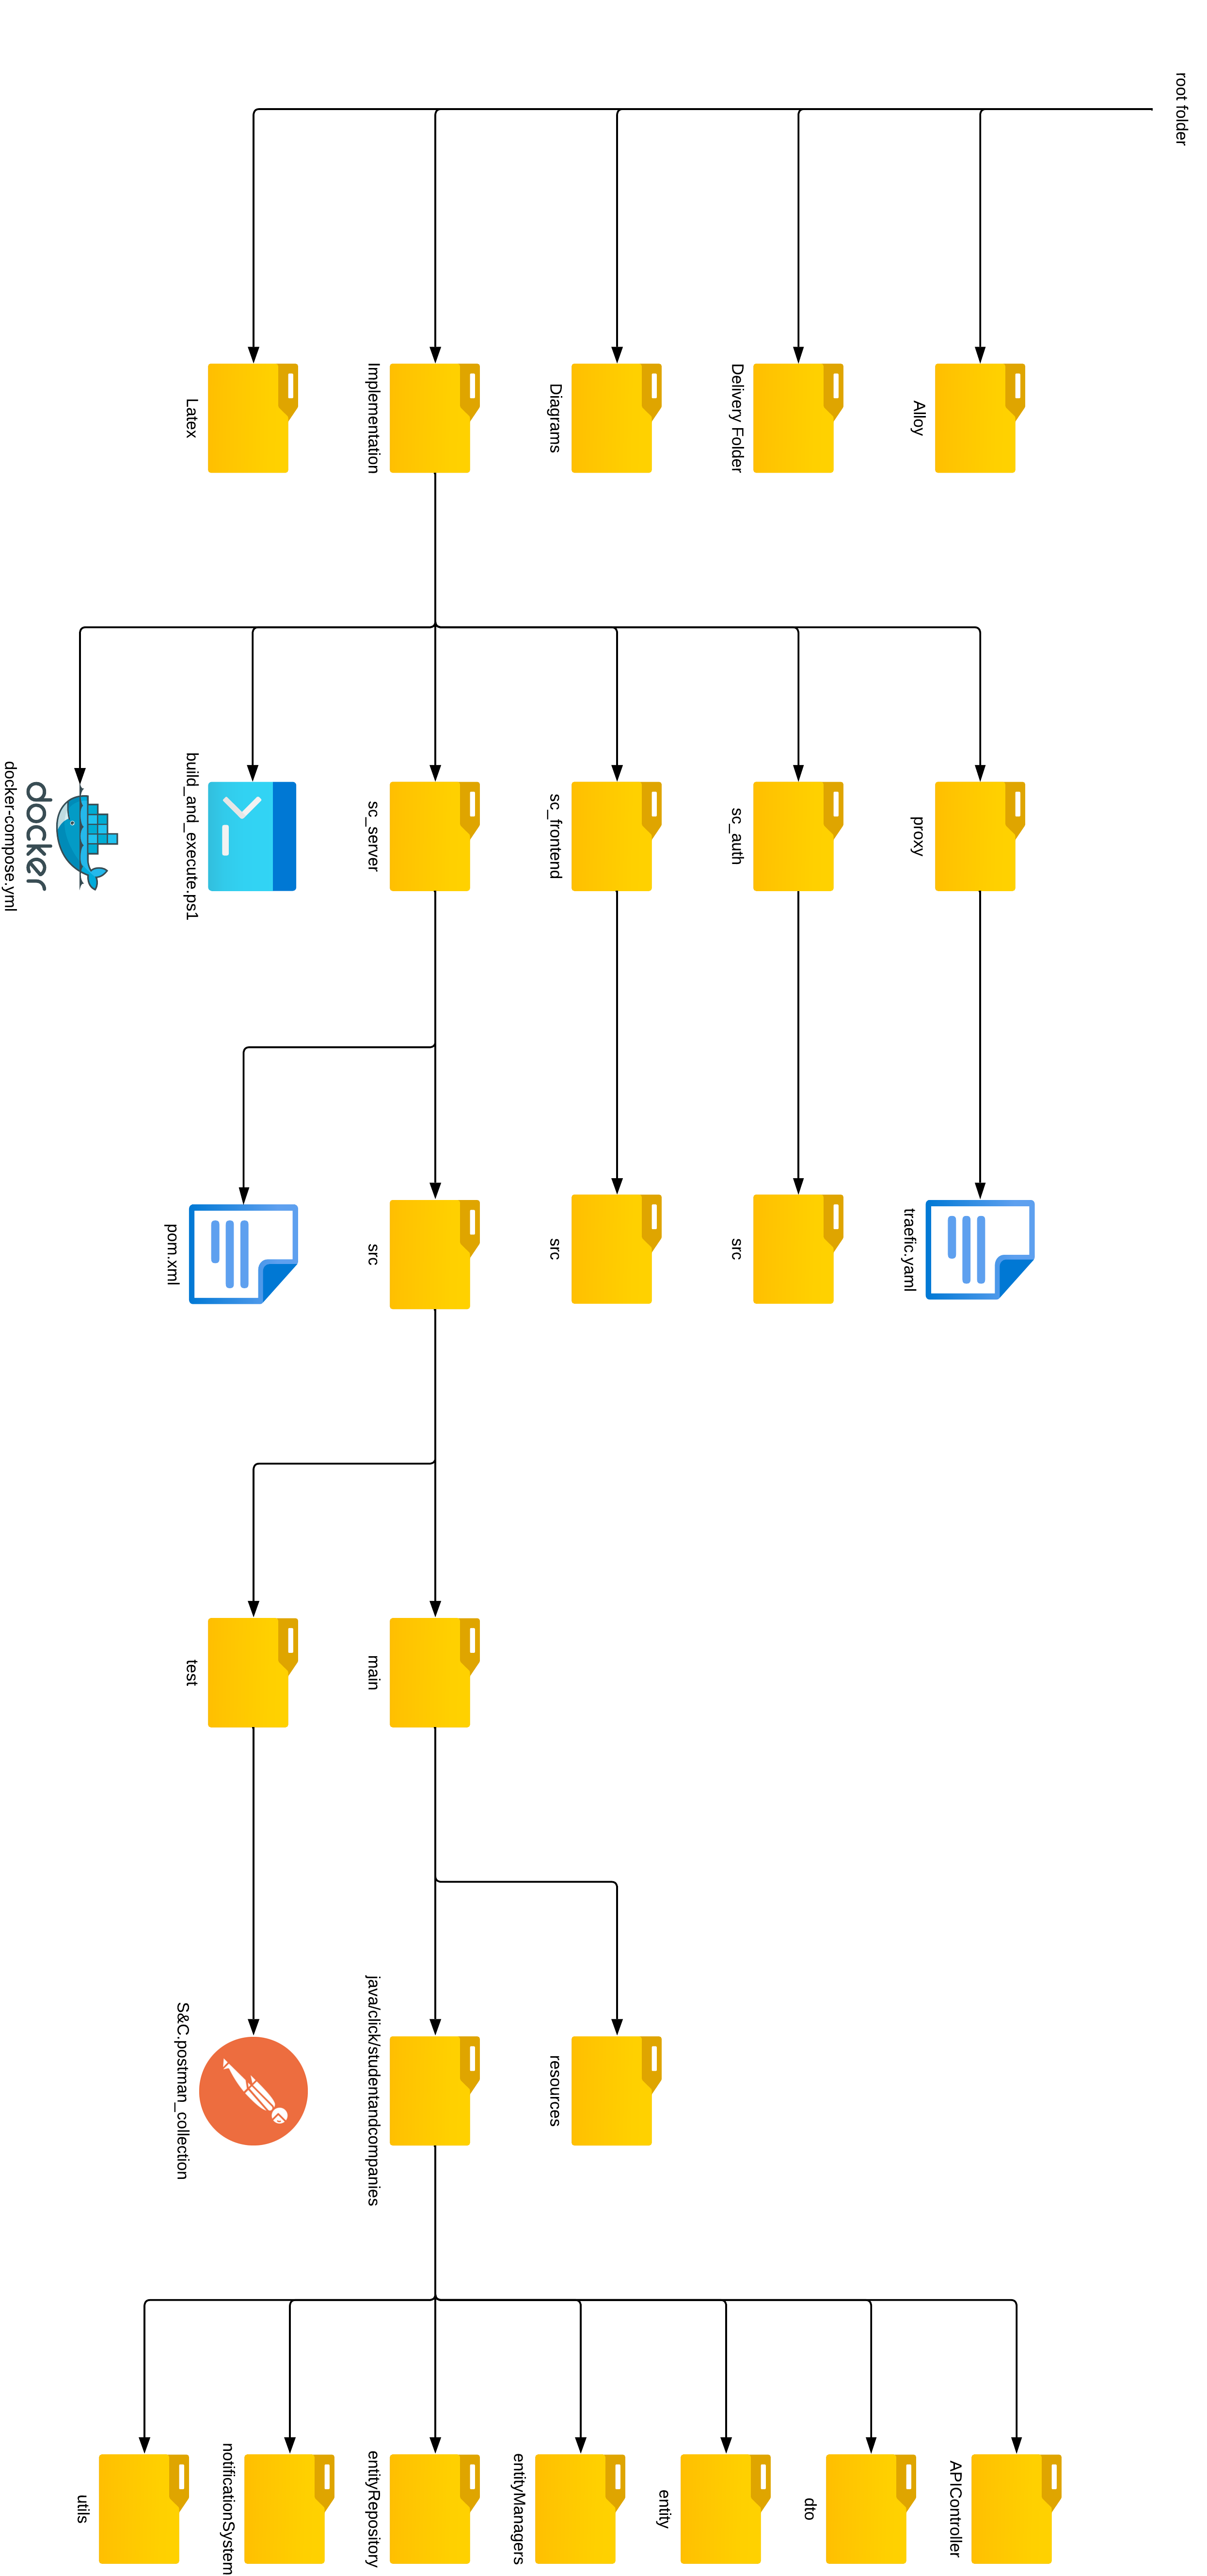
\includegraphics[width=0.55\linewidth]{Latex/Images/ITD/CodeSource.png}
    \caption{Code Source}
    \label{fig:codesource}
\end{figure}
    %------------------------------------------------------------------------------------------------------------------------------------------------
    \clearpage
    \section{Testing Strategy}
    \label{sect:testingstrategy}
    The testing strategy for the S\&C platform is based on a combination of manual and automated testing techniques. Manual testing is performed by the development team to verify the correctness of the application's functionality, user interface, and user experience. Automated testing is performed using testing frameworks and tools to verify the correctness of the application's business logic, data integrity, and performance. The following sections will provide an overview of the testing strategy using during the development and the integration phase.
\subsection{Unit Testing}
For the development testing phase we mainly used JUnit and Mockito to test the backend layer of the S\&C platform. JUnit is a popular testing framework for Java that is widely used in enterprise applications, web development, and mobile applications. Mockito is a mocking framework for Java that allows developers to create mock objects for testing purposes. It is mainly used to isolate the code under test from its dependencies, such as external services, databases, and APIs.\\
Following what we already describe in the DD document, during this phase we mainly focused on testing the business logic of the application and the data integrity. This is visible in the test classes that we created for each of the main components of the S\&C platform which mainly test the CRUD operations of the different entities while postponing the test of the API end-points and the DTO classes to the integration testing phase. 

\begin{figure}[H]
    \centering
    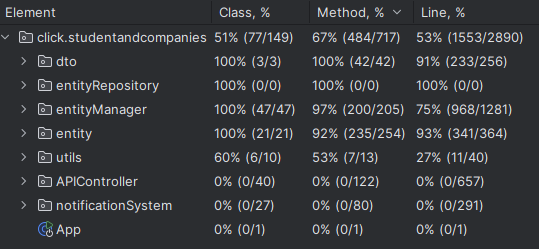
\includegraphics[width=0.5\linewidth]{Latex/Images/ITD/Coverage.png}
    \caption{Coverage result}
    \label{fig:coverage}
\end{figure}

\subsection{Integration Testing}
For the integration testing phase we mainly used Postman as a "Proxy Driver" to test the RESTful APIs created with Spring Boot following the same strategy describe in the DD document at the 3° testing step. The main goal of this phase is to verify that the different components of the S\&C platform work together correctly and that the data flow between them is consistent and reliable. The integration testing phase is performed by the development team to identify and fix any issues related to the interaction between the call made by the frontend and the computation made by the backend and the database. We created more than 30 different API call that were later used in Postman unit suite, that allowed us to test all the different functionalities of the platform, from the user registration to the internship creation, from the recommendation process to the interview management.\\
Postman allowed us to randomize request parameters and body content to test the system's robustness and evaluate different edge cases that could arise during normal platform usage. Examples include creating an internship with a missing field, accepting a recommendation that has already been approved, or attempting to fetch a non-existent internship and much more. The integration testing phase is essential to ensure that the S\&C platform works as expected, all the functionalities are implemented correctly, and the right exceptions are thrown when the user tries to perform an invalid operation.
%insert here postman call screenshot
    %------------------------------------------------------------------------------------------------------------------------------------------------
    
    \clearpage
    \label{sect:installationinstructions}
    \section{Installation Guide}

This section provides the necessary steps to install and run the S\&C platform.

\subsection{Prerequisites}

Before proceeding with the installation, ensure you have the following dependencies installed on your system:

\begin{itemize}
    \item \textbf{Docker}: required to run the backend services with the \verb|docker-compose.yml| file.
    \item \textbf{PowerShell} (Windows users only): optional, but recommended to automate the backend startup process.
    \item \textbf{Node.js and npm}: Required to install and run the frontend application.
\end{itemize}


\subsection{Backend Setup}
\subsubsection*{Docker}

\begin{enumerate}
    \item Ensure Docker is installed and running on your system.
    \item Open a terminal and navigate to the project root directory.

\end{enumerate}
\subsubsection*{Spring .jar Files \& Containerized Environment }

A PowerShell script is provided to create the \verb|.jar| files that will be needed to properly execute the backend services within the docker containers. 

\begin{enumerate}
    \item Open a PowerShell terminal.
    \item Navigate to the "Implementation" directory.
    \item Execute the script: 
    \begin{verbatim}
        .\build-and-execute.ps1
    \end{verbatim}

    \item When prompted, press \textbf{p} for production mode.
    \item Confirm container rebuild by pressing \textbf{yes} when asked.
\end{enumerate}

The script is useful as a shorthand to create the java build files, set up the environment variables and build and execute the containers.

Naturally, the same behavior could be obtained by manually compiling the Maven Java project inside the folders \verb|sc_server| and \verb|sc_auth| with the command \verb|mvn clean package| and then building the containers with \verb|docker compose up --build|



\subsection{Frontend Setup}

\begin{enumerate}
    \item Ensure that \textbf{Node.js} and \textbf{npm} are installed on your system.
    \item Open a terminal and navigate to the frontend directory.
    \item Install dependencies by running:

    \begin{verbatim}
    npm install
    \end{verbatim}

    \item Start the frontend with API support:

    \begin{verbatim}
    npm run dev:api
    \end{verbatim}

\end{enumerate}

\subsection{Final Steps}

Once both the backend and frontend are running, the application should be accessible via the specified local development URL. Make sure both services are properly started before testing the platform.


    %------------------------------------------------------------------------------------------------------------------------------------------------
    
    \clearpage
    \section{Effort Spent}
    \label{sect:effortspent}
    \subsection*{Lorenzo Ricci}
\begin{table}[H]
    \centering
\begin{tabular}{|p{4.5cm}|c|}
        \hline
        \textbf{Unit} & \textbf{Hours} \\ \hline
        Frontend & 99 \\ \hline
        Backend & 20 \\ \hline
        Testing & 5 \\ \hline
        Report & 1 \\ \hline
    \end{tabular}
    \caption{Effort - Lorenzo Ricci}
    \label{tab:effort-ricci}
\end{table}
\subsection*{Matteo Giovanni Paoli}
\begin{table}[H]
    \centering
    \begin{tabular}{|p{4.5cm}|c|}
        \hline
        \textbf{Unit} & \textbf{Hours} \\ \hline
        Frontend & 45 \\ \hline
        Backend & 49 \\ \hline
        Testing & 12 \\ \hline
        Report & 3 \\ \hline
    \end{tabular}
    \caption{Effort - Matteo Giovanni Paoli}
    \label{tab:effort-paoli}
\end{table}

\subsection*{Samuele Grisoni}
\begin{table}[H]
    \centering
\begin{tabular}{|p{4.5cm}|c|}
        \hline
        \textbf{Unit} & \textbf{Hours} \\ \hline
        Frontend & 39 \\ \hline
        Backend & 61 \\ \hline
        Testing & 5 \\ \hline
        Report & 2\\ \hline
    \end{tabular}
    \caption{Effort - Samuele Grisoni}
    \label{tab:effort-grisoni}
\end{table}


    %------------------------------------------------------------------------------------------------------------------------------------------------
    
    \clearpage
    \section{References}
    \label{sect:references}
    % \subsection{Reference Documents} % Sezione numerata per la bibliografia
%     \printbibliography[notkeyword={tools},  heading=none]

\subsection{Used Tools}
    \printbibliography[keyword={usedtools}, heading=none]

\subsection{Reference Tools}
    \printbibliography[keyword={tools}, heading=none]
    %------------------------------------------------------------------------------------------------------------------------------------------------
    
    \clearpage
    \appendix
    \section{Assignement RDD AY 2024-2025}
    \label{appendix:assignement}
    Students\&Companies (S\&C) is a platform that helps match university students looking for internships
    and companies offering them. The platform should ease the matching between students and
    companies based on:
    \begin{itemize}
        \item the experiences, skills and attitudes of students, as listed in their CVs;
        \item the projects (application domain, tasks to be performed, relevant adopted technologies-if any etc.) and terms offered by companies (for example, some company might offer paid internships and/or provide both tangible and intangible benefits, such as training, mentorships, etc.).
    \end{itemize}
The platform is used by companies to advertise the internships that they offer, and by students to look
for internships. Students can be proactive when they look for internships (i.e., they initiate the process,
go through the available internships, etc.). Moreover, the system also has mechanisms to inform
students when an internship that might interest them becomes available and can inform companies
about the availability of student CVs corresponding to their needs. We refer to this process as
“recommendation”.
Recommendation in S\&C can employ mechanisms of various levels of sophistication to match students
with internships, from simple keyword searching, to statistical analyses based on the characteristics of
students and internships.
When suitable recommendations are identified and accepted by the two parties, a contact is
established. After a contact is established, a selection process starts. During this process, companies
interview students (and collect answers from them, possibly through structured questionnaires) to
gauge their fit with the company and the internship. S\&C supports this selection process by helping
manage (set up, conduct, etc.) interviews and also finalize the selections.
To feed statistical analysis applied during recommendation, S\&C collects various kinds of information
regarding the internships, for example by asking students and companies to provide feedback and
suggestions.
Moreover, S\&C should be able to provide suggestions both to companies and to students regarding
how to make their submissions (project descriptions for companies and CVs for students) more
appealing for their counterparts.
In general, S\&C provides interested parties with mechanisms to keep track and monitor the execution
and the outcomes of the matchmaking process and of the subsequent internships from the point of
view of all interested parties. For example, it provides spaces where interested parties can complain,
communicate problems, and provide information about the current status of the ongoing internship.
The platform is used by students at different universities. Universities also need to monitor the situation
of internships; in particular, they are responsible for handling complaints, especially ones that might
require the interruption of the internship.
    
\end{document}
